\chapter{Camera Sensing and Particle Filter}
\section{Important}
Read the entire lab before starting and especially the ``Grading" section as there are points you will receive by completing certain sections or checkpoints by the end of the lab session(s). 

\section{Motivation}
In order to design an intelligent robot to effortlessly carry out tasks, the robot must first be able to estimate a ``state" from sensor data.  For example, if a robot needs to navigate a path out of a room, it first must figure out where it is relative to the exit.  If an autonomous car wants to avoid a pedestrian, it first must gather detection data and figure out the relative position of the person. If we had perfect knowledge of the world, determining what to do is relatively straightforward. Unfortunately, there is a great deal of uncertainty (noise) in our sensors (and most robot environments), and most variables are not directly measurable. 
\\* 
\\* State estimation is meant to address the problem of estimating quantities that are not perfectly or directly observable from sensor data.  By gathering sensor data, we can design a state estimation scheme that can recursively update it's belief of the true state variables from the data. In this lab, you will implement a standard technique for localization, which will help the UR3 find itself in a maze.  
\\* 
\\* So with this lab we are taking a leap ahead in what you know about moving a robot arm from one position (state) to another position. In fact, we will be giving you code libraries that you you will be developing for yourself in Lab 4 and Lab 5. We are doing things in this order to give you motivation for all the linear algebra and geometry you will need to solve to develop labs 4 and 5.  So you will not yet know how to move the robot from one position to the next but we will be giving you code to step the robot from one grid position to the next position.  
\\* 
\\* Our first step in this lab is to measure the location (or state) of the end effector of the robot arm.  You will be placing an orange circle at the end of the robot arm and you should think of this as a point that needs to move around a grid course in the camera's field of view.  For this exercise we are not worried about whether the arm links position over the grid walls, we are only interested in the orange circle's position.  
\\* 
\\* When trying to understand the pose or state of a robotic system, it is always important to keep in mind the error in the measurements and model of the system.  In the homework particle filter simulation, noise is added to simulate this error.  For our actual implementation we are going to use the camera installed above your robot's bench as our measurement of where the robot (orange disk) is located.  This of course will introduce error in the measurement so the actual run will not have to add noise to the measurement.  
\\* 
\\* Besides working with the particle filter in this lab, another important aspect of this lab is introducing you to the \textbf{OpenCV} computer vision library.  For this lab we will be asking you to just use the \textbf{simpleBlobDetector} algorithm to find centroids of orange blobs.  In lab 6 you will again be asked to use openCV to find centroids and that task can probably be done with \textbf{simpleBlobDetector} again.  It is the hope of this lab though to show you that simple web searches of openCV topics can show you other algorithms/techniques to perform similar tasks.  In lab 6 you will have the freedom to experiment more with openCV and even change the lab assignment to your liking to solve a different but similar problem than the one assigned. This will allow you to experiment with other algorithms/functions of openCV.

\section{Objectives}
\begin{itemize}
    \item Become more familiar with ROS.
    \item Introduce the computer vision development library, \textbf{OpenCV}. 
    \item Use the OpenCV class \textbf{simpleBlobdetector} to find the centroid of orange ``blobs”.  
    \item Find the transformation from camera pixel coordinates to robot world coordinates and then in the final exercise transform to maze coordinates. 
    \item Implement the same particle filter exercise assigned in homework but now instead of simulating the measurement of the orange blob/turtle robot's state use the camera to measure the coordinates (state) of the robot's position. 
\end{itemize}

\section{References}
\textbf{HSV Color Space:}
\begin{itemize}
\item \url{https://en.wikipedia.org/wiki/HSL_and_HSV}
\item \href{https://stackoverflow.com/questions/10948589/choosing-the-correct-upper-and-lower-hsv-boundaries-for-color-detection-withcv}{https://stackoverflow.com/questions/10948589/}
\end{itemize}

\textbf{Simple Blob detector:}
\begin{itemize}
\item \url{www.learnopencv.com/blob-detection-using-opencv-python-c/}
\item \href{https://stackoverflow.com/questions/8076889/}{https://stackoverflow.com/questions/8076889/how-to-use-opencv-simpleblobdetector}
\item \url{https://www.programcreek.com/python/example/89350/cv2.SimpleBlobDetector}
\item \url{https://www.programcreek.com/python/example/71388/cv2.SimpleBlobDetector_Params}
\end{itemize}

\section{Tasks}
\begin{itemize}
\item Use the USB camera and the \textbf{OpenCV} library's \textbf{simpleBlobDetector} class to find “blobs” of orange color and locate their center coordinates in pixels.

\item Determine the perspective transform of the camera. -- Find the transformation matrix that transforms the centers found by the camera in pixels coordinates (row,column) to World robot coordinates $(x_w,y_w)$ in meters.  
Normally perspective transform involves finding the intrinsic, extrinsic, and distortion parameters that describe the mapping between 3D world points to 2D image points.  For our purposes we 
will make several assumptions that will vastly simplify the transformation:\\
\begin{itemize}
	\item The image plane is always parallel to the table ($z_w$ and $z_c$ are parallel).
	\item The yaw angle difference between the world coordinates and camera coordinates is considerably small ($x_w$ and $x_c$ are almost parallel).
	\item Fish eye distortion of the camera has been corrected.
\end{itemize}


\setlength{\parskip}{10pt}
Several parameters must be specified in order to implement the equations.  Specifically, we are interested in $\theta$ the rotation 
between the world frame and the camera frame -- which is expected to be fairly small since we aligned the camera before each lab section. $\beta$, the scaling constant between distances in the world frame and distances in the 
image.  We will compute these parameters by measuring object coordinates in the world frame and relating them to their corresponding 
coordinates in the image.
\setlength{\parskip}{0pt}

\item Use the measurement of the center of the orange disk attached to the robot's end effector as the measurement of the object traversing the maze of your particle filter homework.  Now instead of knowing exactly where the vehicle (orange blob) is in the maze you will be measuring the state of the vehicle using the above camera.  
\end{itemize}


\section{Procedure}

\subsection{Threshold camera image to distinguish only bright orange pixels}

\begin{enumerate}

\item Starter code for Lab 3 is given at the lab website \url{coecsl.ece.illinois.edu/ece470} under Lab 3. Download this \textbf{tar.gz} file to your catkin directory’s \textbf{src} folder and then extract. 

Explore into the \textbf{lab3pkg\_py/scripts} folder and double check the properties of \textbf{lab3\_image\_tf\_exec.py}, \textbf{lab3\_image\_exec.py} and \textbf{lab3\_move\_exec.py} are set to executable.  

\item Open a terminal window, change to your catkin directory and run \textbf{catkin\_make}. 

 
\item Now you can run the starter code. 

\begin{lstlisting}[language=bash]
$ source devel/setup.bash
$ roslaunch ur3_driver vision_driver.launch
\end{lstlisting}

Open a second terminal window

\begin{lstlisting}[language=bash]
$ source devel/setup.bash
$ rosrun lab3pkgpy lab3_image_tf_exec.py
\end{lstlisting}

You should see two Windows open.  One is the camera’s video with an added horizontal black line and small red circle.  Later in this lab you will use the horizontal line to straighten the mounting of the camera if it got moved or bumped.  For the red dot towards the top left corner of the image look at the text printing in the terminal.  A three number (H,S,V) value is printing.  You can use this pixel value to help you find the range of H,S,V (Hue, Saturation, Value) values for an orange color. 

\textbf{Side Note:}  What is the H,S,V color space?  Please see the reference link to the Wikipedia  page discussing color spaces.  You are probably most familiar with the R,G,B (red,green,blue) color space.  Here each pixel of an image has a R,G,B value.  With H,S,V colors are placed on a color wheel and you indicate which color you are interested in by selecting an angle range.  In \textbf{OpenCV} the range of the angle is from 0 degrees to 180 degrees.  (You will find other implementations that use 0-360).  For example a blueish color would be in the angle range of 110 degrees to 130 degrees.  The S value is a number between 0 and 255 with 0 being very white and washed out and 255 the full, clear color.  The V value is also a number between 0 and 255 with 0 being very dark and shaded and 255 the full clear color.  The main reason we use the H,S,V color space in this lab is that it makes finding a color with different shading and lighting conditions much easier. 

\item At this point take a look at the given python files in the \textbf{lab3pkg\_py/scripts} folder. This section will only be modifying the files \textbf{lab3\_func.py} and \textbf{lab3\_image\_tf\_exec.py}.  Take a look at these two files.  Notice in \textbf{lab3\_func.py}, in the function \textbf{blob\_search}, the code is converting the RGB image to HSV.  Then using a range for blueish pixels the \textbf{inRange} function is used to threshold/mask the image to a binary image of only blueish pixels. (Binary image means all blueish pixels are ones and all other pixels are zeros).  Next the masked image is cropped to only use the portion of the image that views the maze.  (You will adjust the size of this cropped image in a few steps).  Then at the bottom of the function both the color image and the cropped binary image are displayed in separate windows.  (Notice in those windows there is a button that allows you to save the current image to a file.)
  
\item So your first goal is to find the range of Hue, Saturation and Value that allows your program to find the orange circle in all spots of the camera’s view.  To find these HSV ranges you will need to do some trial and error.  You are supplied with two tools to help you find the correct range.  One is the red dot printed for you on the camera’s video frames.  Notice that when you put a colored block or the orange circle under that red dot the terminal window prints out the H,S,V value for that pixel.  Experiment with a few colors and see the H,S,V values change.  The code for putting this red dot on the image and displaying the H,S,V values to the terminal is in the \textbf{lab3\_func.py} file towards the end of the \textbf{blobsearch} function.  The \textbf{cv2.circle} function is used to add the red dot and the print statement prints out the H,S,V values.   
One issue with this method is that it only shows one pixel and therefore only one lighting condition.  You need to make sure your range of H, S, V values work in all areas of the cropped image.  So going on from here, you need to do some trial and error.  Pick a range for H and S and V, change your code with that range and see how well the cropped image shows only the orange disk in all of its area.  We have also supplied you with some off line code, \textbf{HSV.py}, that takes a single picture file and prints out a H,S,V range for the pixels selected.   

	\begin{figure}[h]
	\centering
		
\includegraphics[height=1cm]{lab3_cam_cali7.png}
	\caption{\figlbl{3cali7} How to snapshot the video feed.}
    \end{figure}

\item Once you have found a good H,S,V range for the orange disk and your benches lighting conditions, you need to make sure the cropped image views all the area of the maze.  First step is to look at the full color image and make sure the camera is turned so the black horizontal line is also horizontal with respect to the robot’s base.  Have your TA help you with this.  (Of course try your best not to bump the camera so that this process does not have to happen too often.).  Then return to looking at the cropped binary image and move the orange disk to all corners of the maze.  Make sure that the orange disk is seen in the cropped image at all the corners.  If the cropped image does not see all corners of the maze you will need to modify the values \textbf{crop\_top\_row}, \textbf{crop\_bottom\_row}, \textbf{crop\_top\_col} and \textbf{crop\_bottom\_col} to move where the top and bottom corners of the cropped image are located.  Note that the full image size is 480 rows by 640 columns.    

\end{enumerate}
		
\subsection{Use the OpenCV simpleBlobdetector library function to find the centroid in pixels of one or multiple circular orange blobs}

\begin{enumerate}

\item At this point you need to do a bit of reading at the \textbf{OpenCV} websites listed in the Reference section and perform your own web search to figure out how use \textbf{OpenCV}’s \textbf{simpleBlobdetector} library.  Part of the goal of this assignment is learn \textbf{OpenCV} and use web searches to find examples of different library functions. 

For this lab you should only us the \textbf{simpleBlobdetector} algorithm but in Lab 6, if you wish, you will be allowed to use additional \textbf{OpenCV} features to recognize objects seen by the camera.  You are given starter code to get you started with \textbf{simpleBlobdetector}.  See in \textbf{lab3\_func.py} the function \textbf{blob\_search\_init}.  This is where you need to set the parameters for \textbf{simpleBlobDetector}.  By default all the “filterBy…” parameters are set to False.  You need to decide which of these filters will work best to find the orange disks in the cropped image.  There are also other parameters you will need to set in this function which are not given to you.  Once you think you have set all the correct parameters, switch to the \textbf{blob\_search} function and find the comment that shows you where to call the “detect” method of \textbf{simpleBlobDetector}.  

The detect method returns \textbf{keypoints}, which is a variable that has the centroid and other information of each blob found.  If there is only one orange blob then \textbf{keypoints} only has one element.  If there are more blobs then \textbf{keypoints} also has the centroids for those blobs.  The web pages listed in the References section show example code of getting information out of the \textbf{keypoints} variable.  Use the \textbf{print()} function to print out the number of blobs found and the coordinates of the first blob.  Also use the \textbf{cv2.drawKeypoints()} function to draw a circle around each blob in the color video frames. \textbf{simpleBlobDetector} is being passed the cropped image.  The centroid found is in pixel units.  (0, 0) is the top left corner of the cropped image.  Therefore you will need to add \textbf{crop\_top\_row} and \textbf{crop\_top\_col} to the \textbf{Keypoint}'s centroid values before calling the \textbf{cv2.drawKeypoints()} function with the full color image.  \textbf{Keypoints} is a list of the \textbf{Keypoint} class.  One of the elements in the \textbf{keypoint} class is pt, which is a tuple.  To modify an element in a tuple, first change the tuple to a list with the \textbf{list()} function.  Modify the element of the newly created list and finally set the \textbf{Keypoint.pt} tuple element to the modified list by converting the list to a tuple with the \textbf{tuple()} function. Figuring out the correct parameters for \textbf{simpleBlobDetector} will take some trial and error.

\item Using two orange disks, move them to many different locations in the maze and print out the centroids found.  Make sure that these centroids make sense in pixels where the (0, 0) camera origin is the top left corner. 

\end{enumerate}


\subsection{Perspective Transform} \label{CamCal}
\begin{enumerate}
	\item Read appendix C.3 before proceeding further.

\begin{figure}[h]
	\centering
		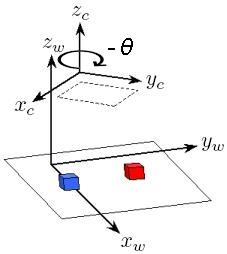
\includegraphics[height=6cm]{lab3_calibrate1.jpg}
	\caption{\figlbl{3cali1} Arrangement of the world and camera frames.}
\end{figure}

	\item Begin by writing the equations we must solve in order to relate image and world frame coordinates.  You will need to combine the 
intrinsic and extrinsic equations for the camera; these are given in appendix C.3.  Write equations for the world frame coordinates in terms of the image coordinates.
	\begin{eqnarray*}
		x_w(r,c) & = & \\
		y_w(r,c) & = &
	\end{eqnarray*}
	
	\item There are six unknown values you must determine: $O_r, O_c, \beta, \theta, T_x, T_y$.  The principal point $(O_r,O_c)$ is given by the row and column coordinates of the center of the image.  We can easily find these values by dividing the \texttt{width} and \texttt{height} variables by 2.
	\begin{eqnarray*}
		O_r & = & \frac{1}{2}height = \\
		O_c & = & \frac{1}{2}width =
	\end{eqnarray*}
	
	\begin{figure}[h]
	\centering
		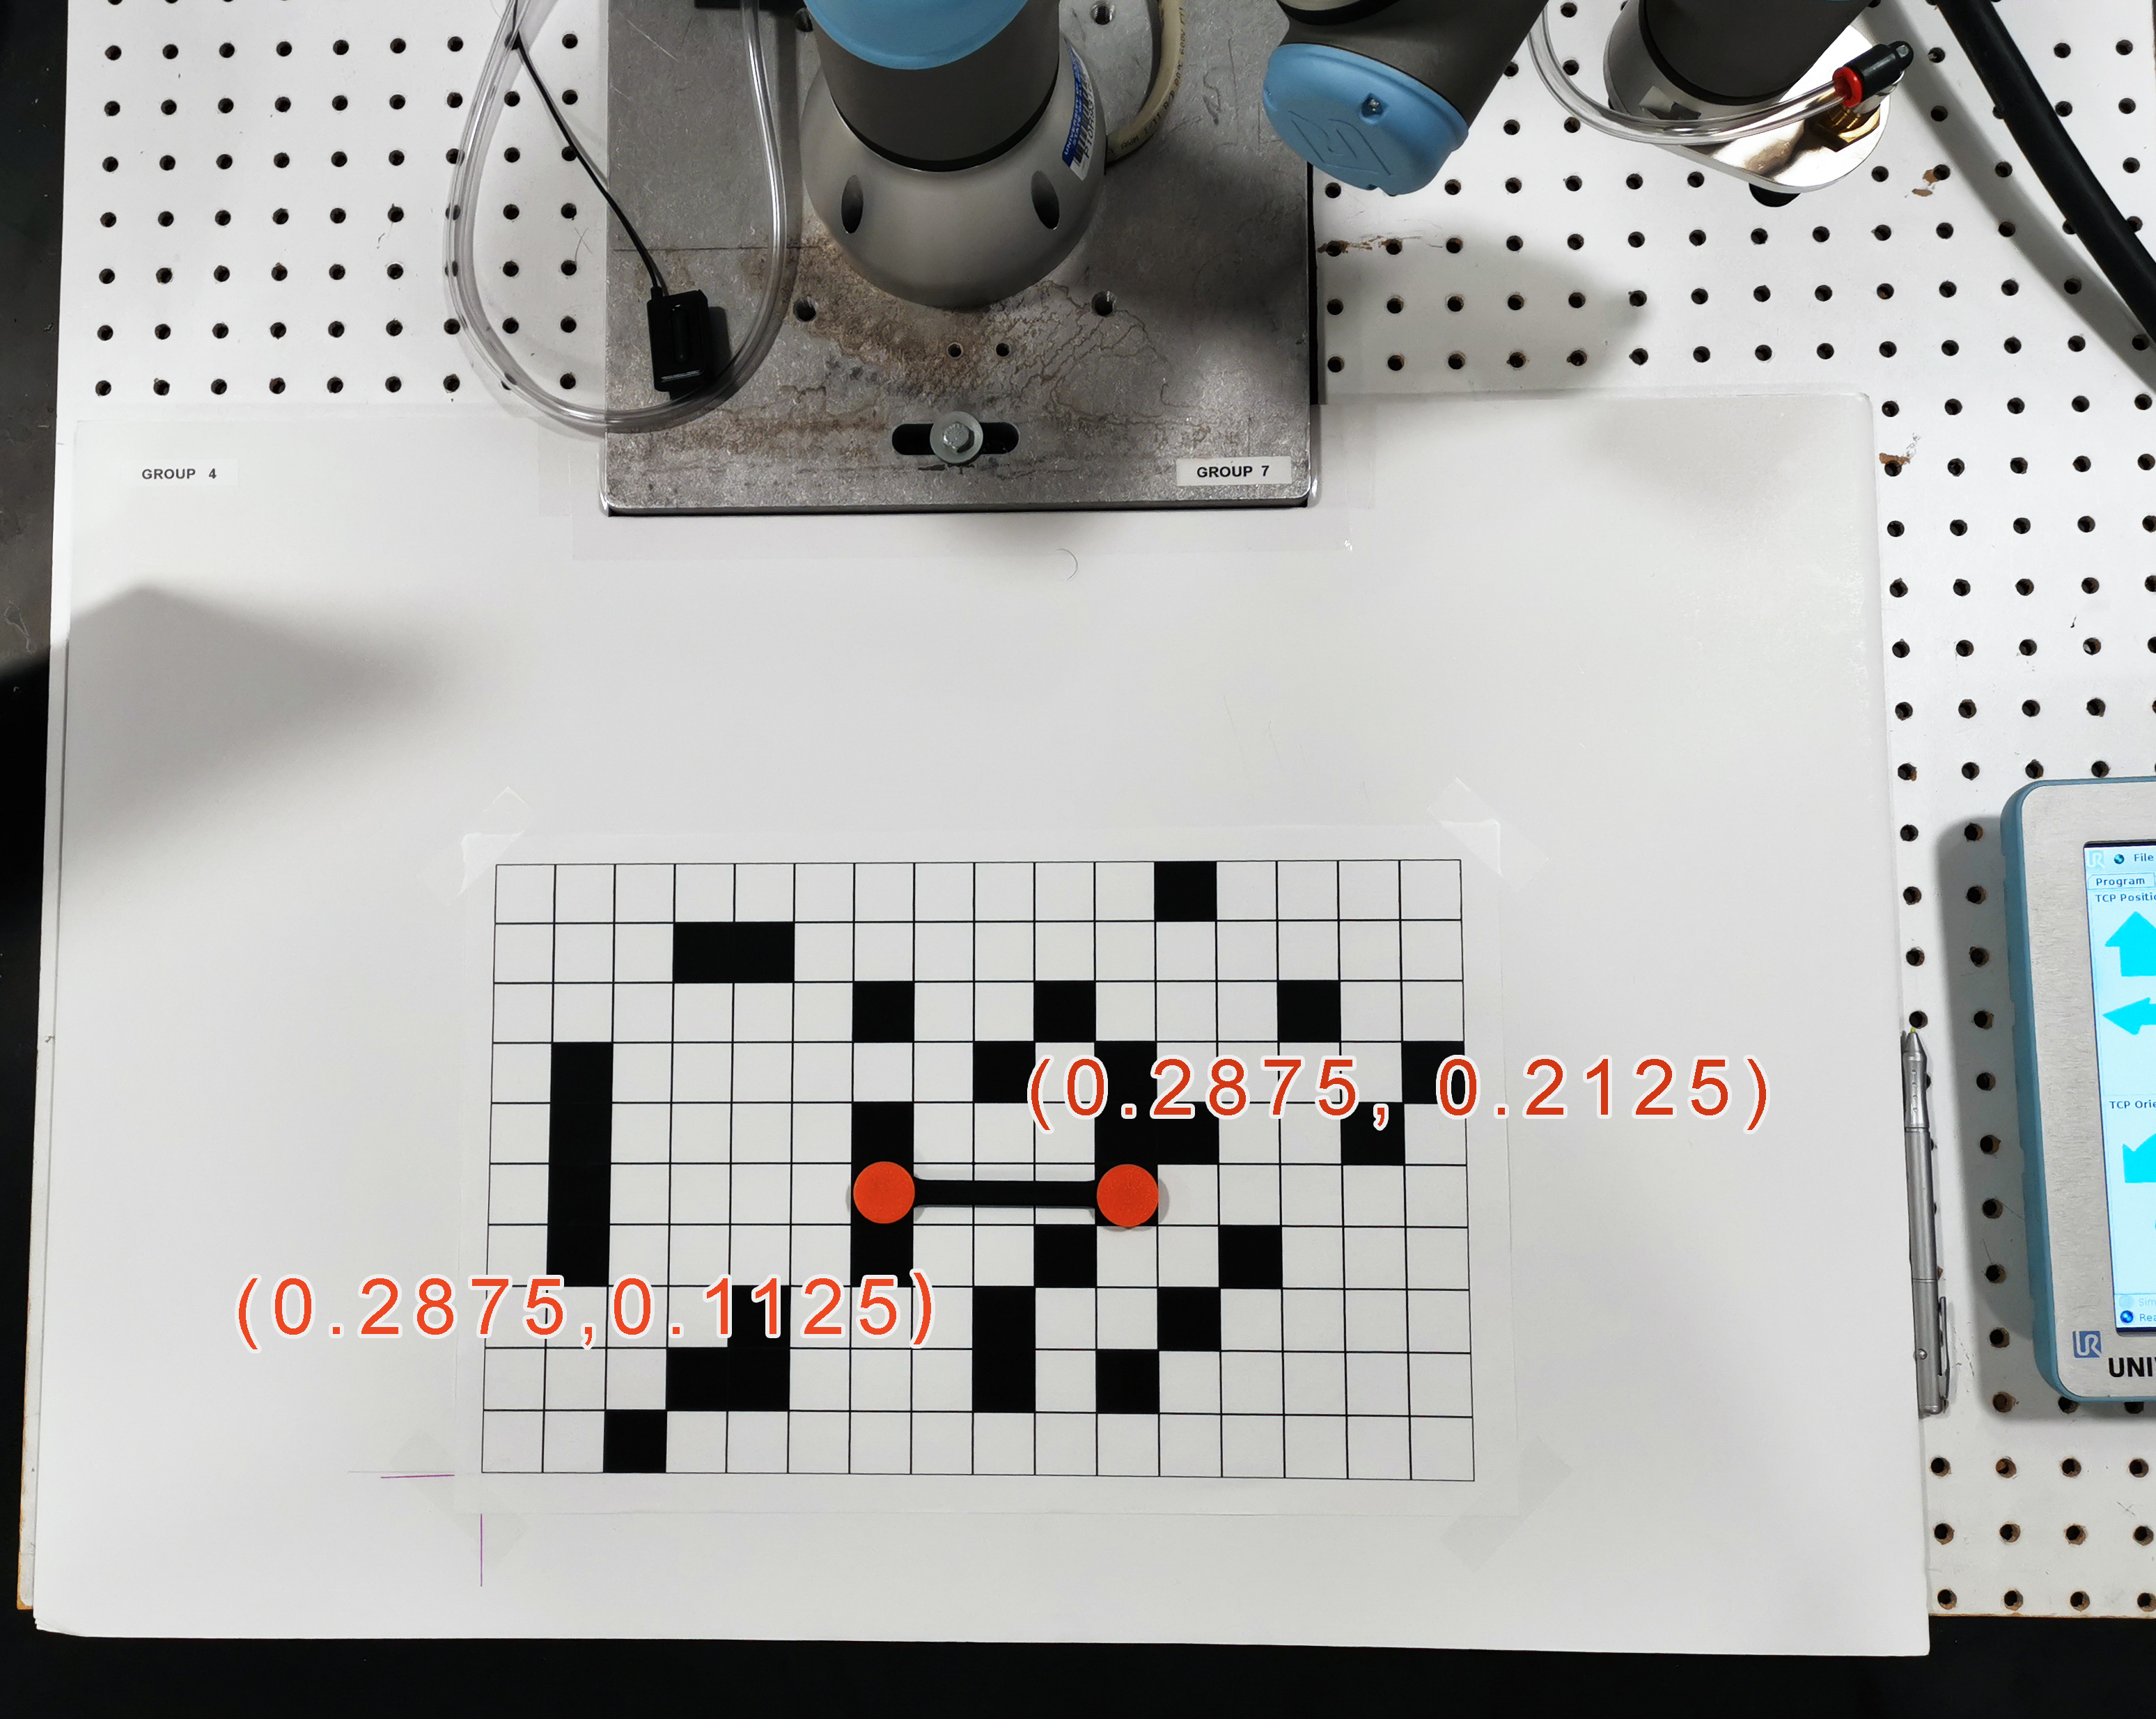
\includegraphics[height=8cm]{lab3_cam_cali6.jpg}
	\caption{\figlbl{3cali6} Where to place the calibration stick.}
    \end{figure}
	
	You will calculate the parameters $\beta, \theta, T_x, T_y$ in the python script:
	
	\textbf{lab3\_image\_tf\_exec.py}
	
	First, place the calibration stick in the position ($x_w = 0.2875$, $y_w = 0.1125$ and $x_w = 0.2875$, $y_w = 0.2125$) shown in the \figref{3cali6}. Please keep anything orange (including your hands) away from the camera's field of view. 
	Open a terminal window:
	
	\begin{lstlisting}[language=bash]
    $ source devel/setup.bash
    $ roslaunch ur3_driver vision_driver.launch
    \end{lstlisting}
    
    Open a second terminal window:
    
    \begin{lstlisting}[language=bash]
    $ source devel/setup.bash
    $ rosrun lab3pkgpy lab3_image_tf_exec.py
    \end{lstlisting}
	
    You will modify this code (which will print these values to the terminal by default as zeros) to calculate $\beta, \theta, T_x, T_y$ values so that you can use them in \textbf{lab3\_image\_exec.py}.
	
	Note that you may have to rerun this procedure to obtain these values when you return to the lab, as other groups will be using the same camera and may re-position the camera when you are not present. To keep these values relatively consistent, \textbf{PLEASE TRY NOT TO BUMP OR MOVE THE CAMERA.}
	
	$\beta$ is a constant value that scales distances in space to distances in the image.  That is, if the distance (in unit length) between two points in space is $d$, then the distance (in pixels) between the corresponding points in the image is $\beta d$. Note that the calibration stick is exactly 0.1 m long.
	\[
	\beta =
	\]
	
    \begin{figure}[t]
	\centering
	\begin{tabular}{cc}
		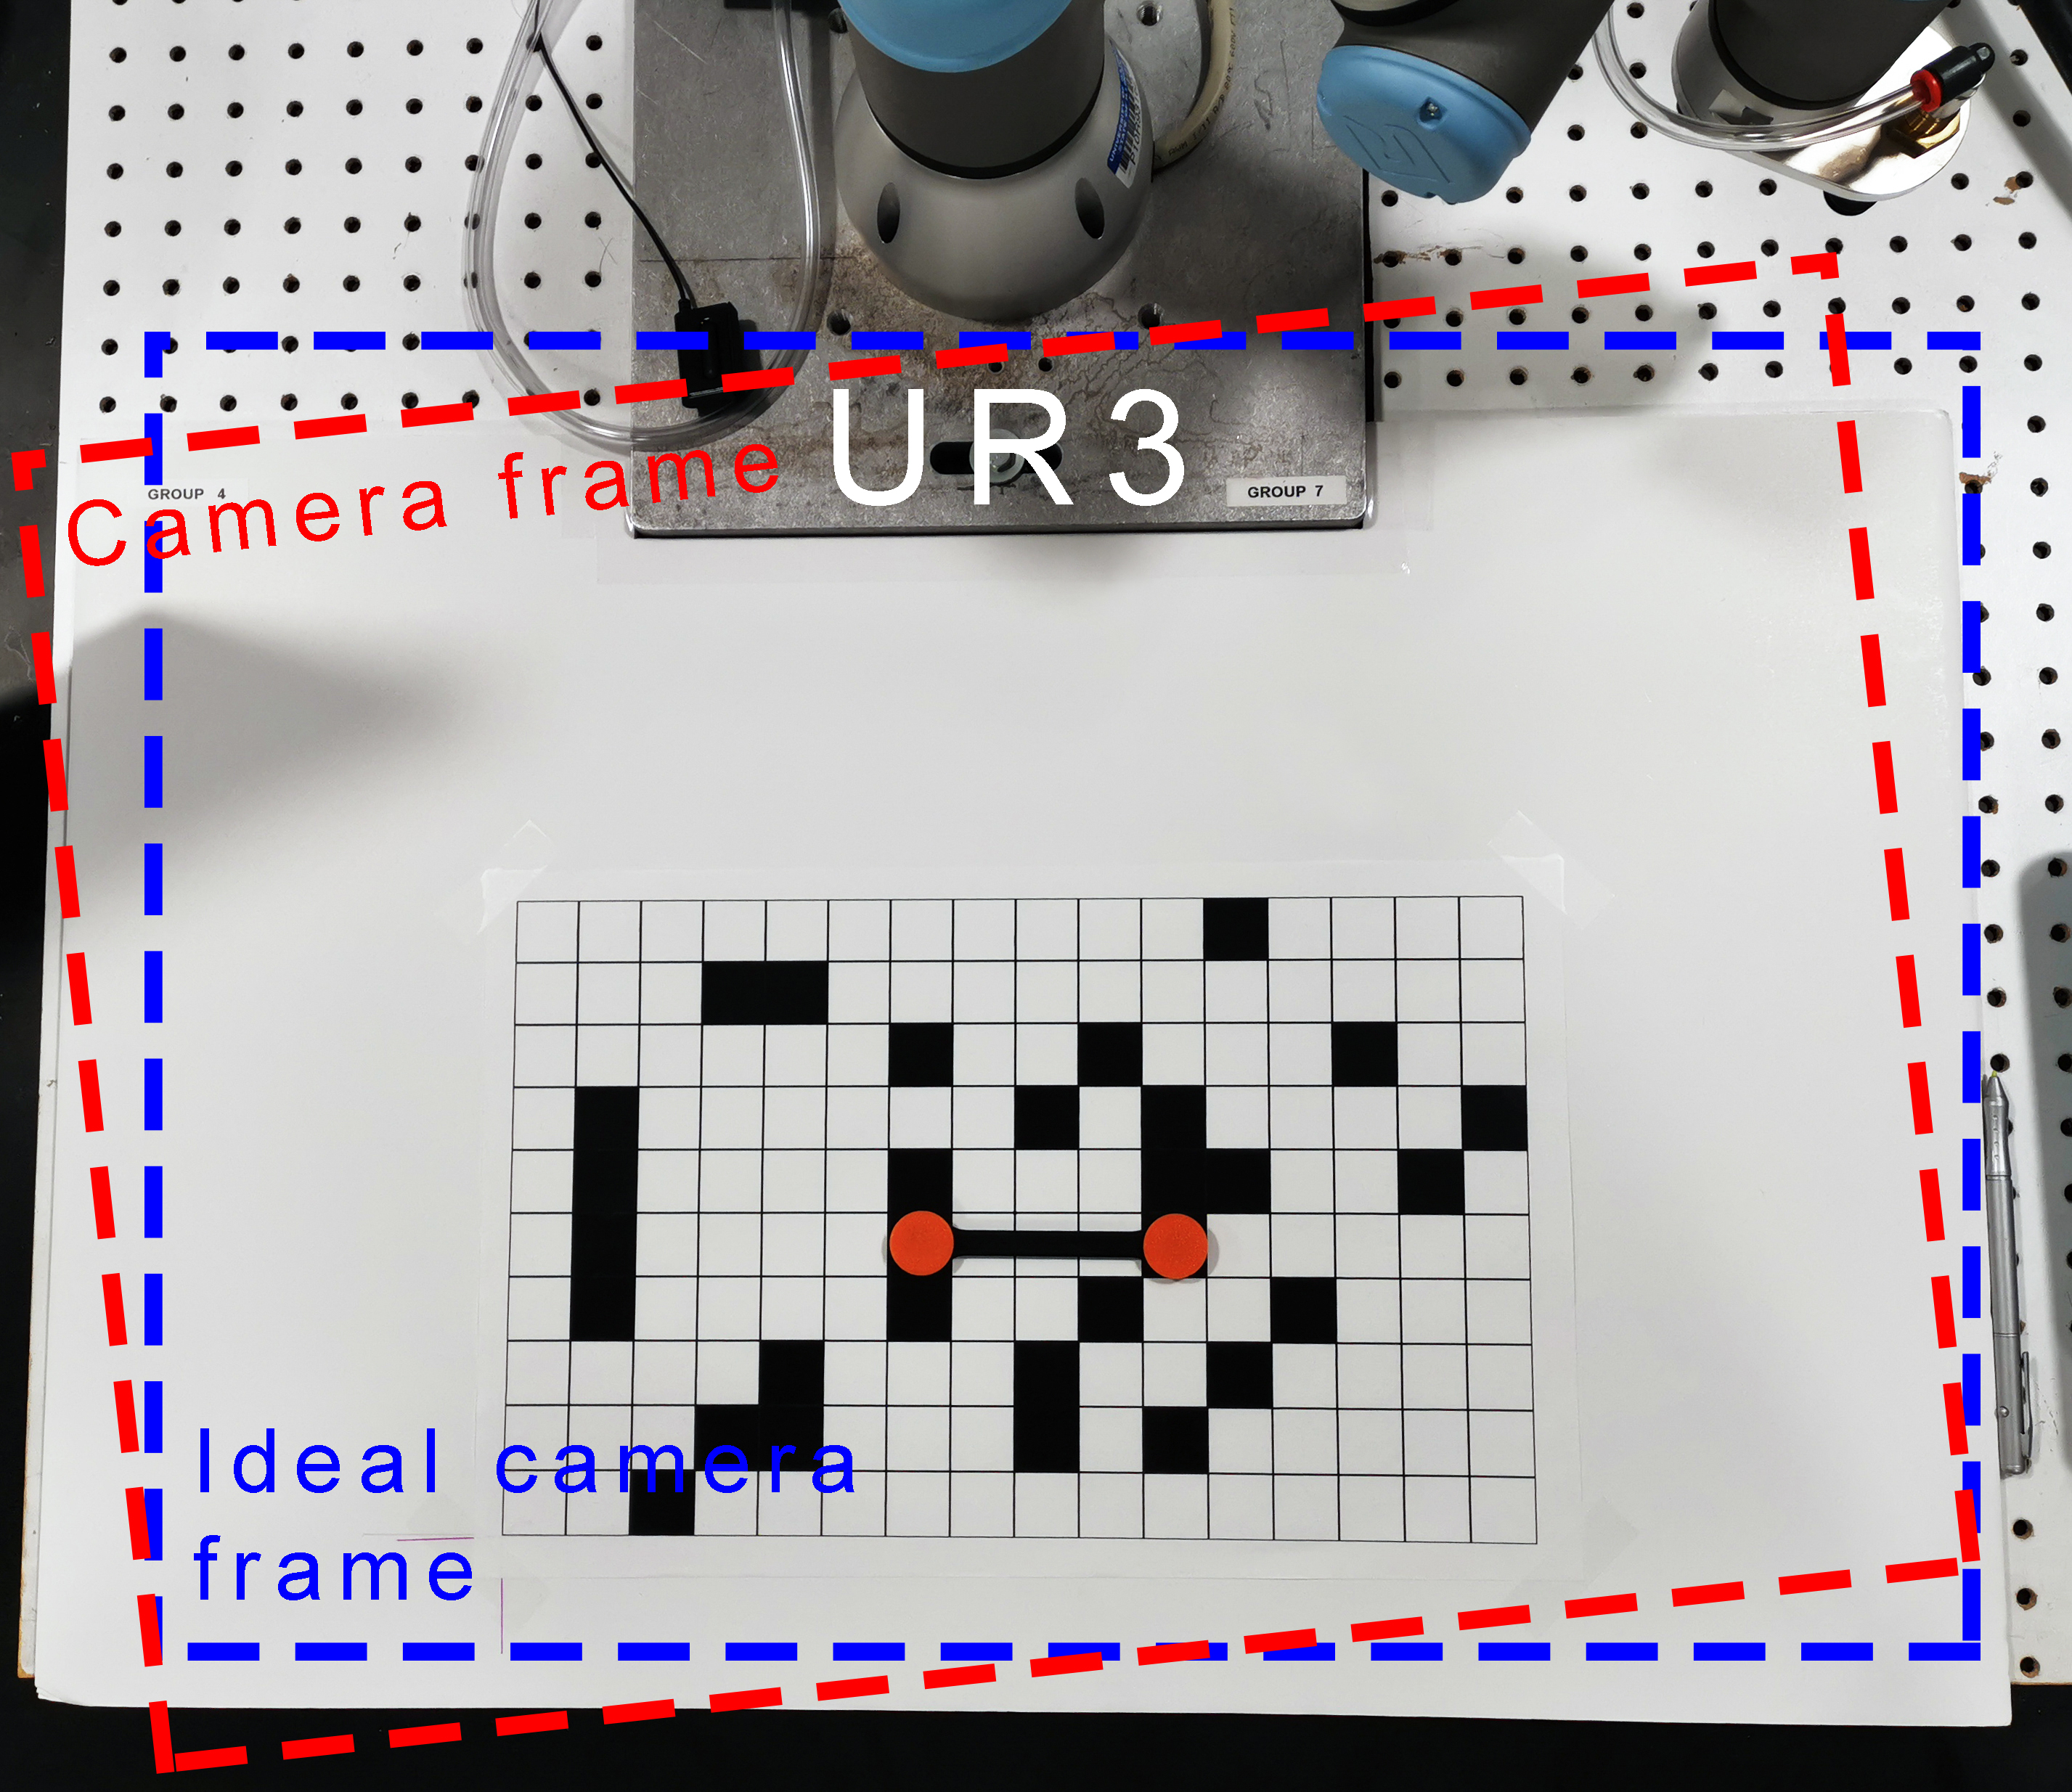
\includegraphics[height=5.5cm]{lab3_cam_cali2.jpg}	&  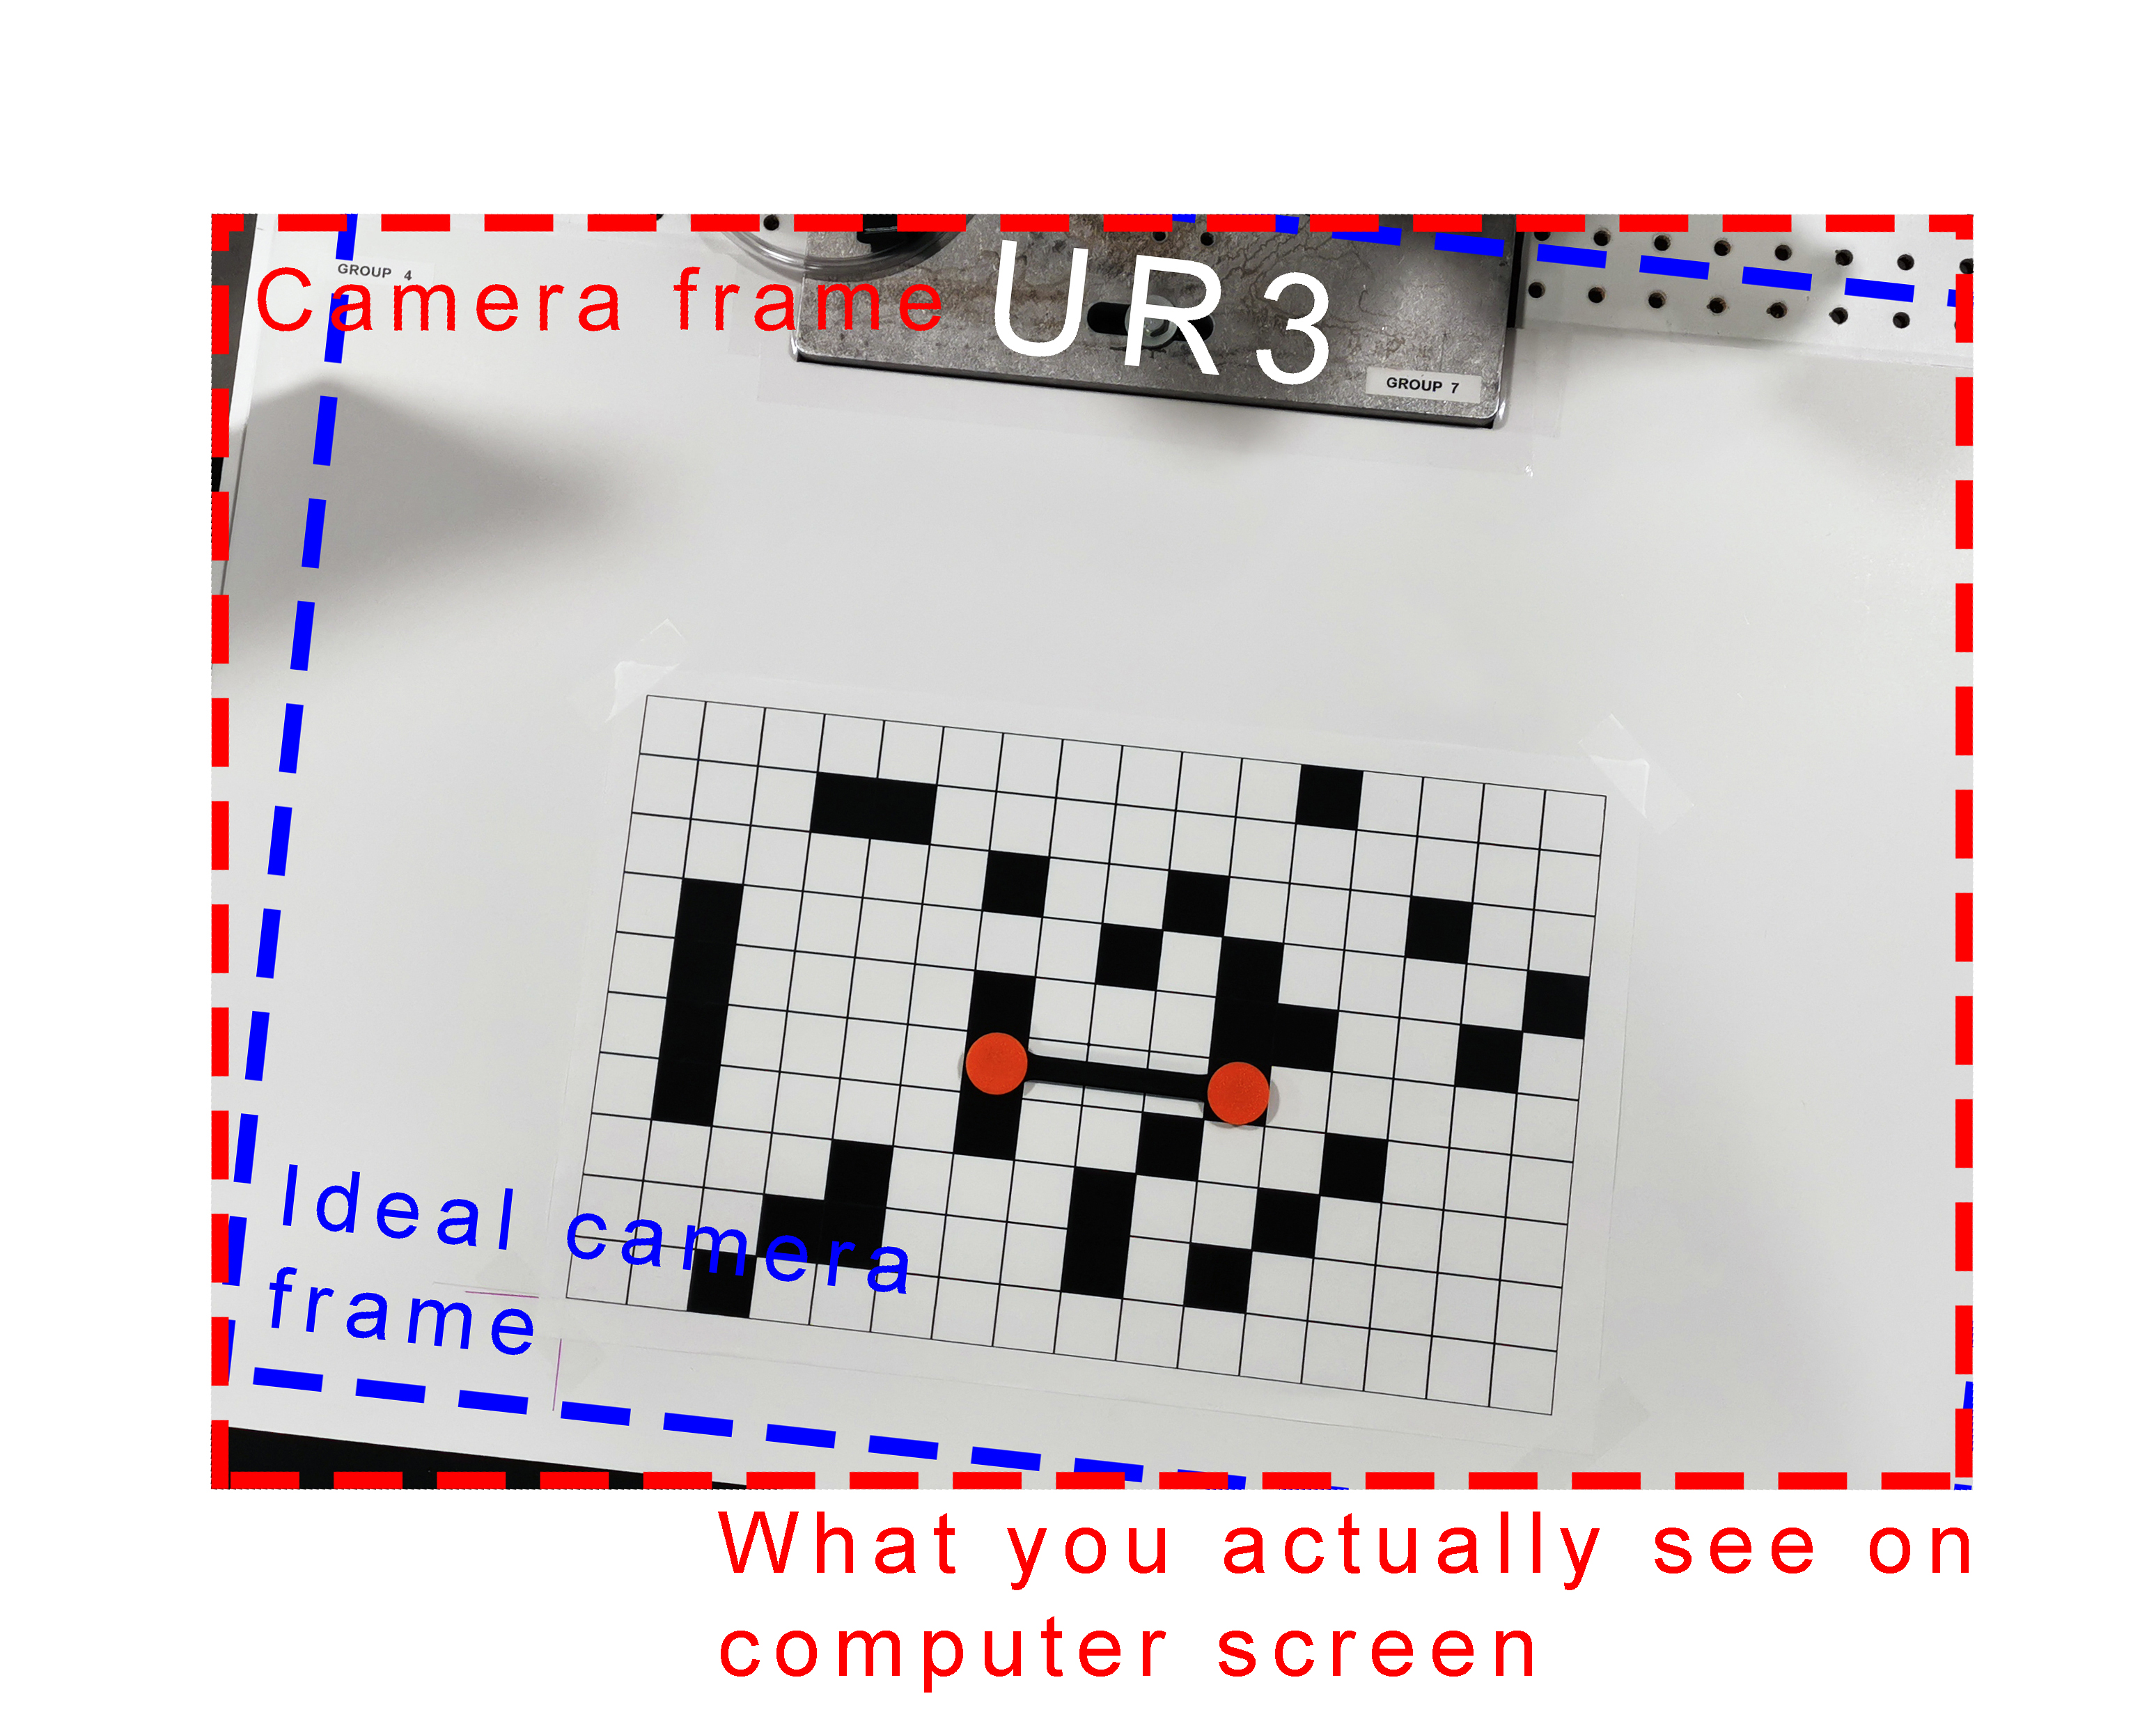
\includegraphics[height=5cm]{lab3_cam_cali3.jpg} \\
		(a) & (b)\\
	\end{tabular}
	\caption{\figlbl{3cali2} (a) Overhead view of the table; the rectangle delineated by blue dashed lines represents the desired camera's field of view, while the red dashed lines represents the actual camera's field of view  (b) The actual image seen by the camera.  Notice that $x_c$ increases with increasing row values, and $y_c$ increases with increasing column values.}
    \end{figure}

	$\theta$ is the angle of rotation between the world frame and the camera frame. \figref{3cali2} gives an overhead view of the blocks with a hypothetical cutout representing the image captured by the camera.  Because the camera's x and y axes are not quite parallel to the world x and y axes, the blocks appear rotated in the image. You may expect this parameter to be fairly small.

	\[
	\theta = 
	\]
	
	$T_x, T_y$ (unit in meters), the origin of the world frame expressed in the camera frame. 
	
	Substitute these values into the two equations you derived in step 2 above and solve for the unknown values.
	\begin{eqnarray*}
		T_x & = & \\
		T_y & = & 	
	\end{eqnarray*}
	
\end{enumerate}

\subsection{Implement particle filter HW problem with real world vision measurements}
This section of the lab is an extension of the particle filter homework problem assigned in lecture.  You will need to have the homework problem completed before attempting this section.  In the homework problem, the location of the turtle was the center of a grid with some additional noise added to the position to make the simulation a bit more realistic.  Using the USB camera viewing the robot’s work environment, we will introduce a measurement of the x, y position of a point at the end of the robot’s gripper.  
The below steps will walk you through moving your python code from your homework code into the \textbf{lab3\_move\_exec.py} file.  These are the “TODO” sections of the homework. 
\begin{enumerate}
\item The \textbf{Maze} class does not need any changes or additions
\item The \textbf{default\_2D\_Model} class also needs no changes but do note that there is a change from the homework with the \textbf{readingSensor} function.  \textbf{readingSensor} is now passed the camera measured centroid of the detected orange blob.  
\item In the \textbf{particleFilter} class \textbf{\_\_init\_\_} function add your code to create the initial set of particles and weights.  
\item In the \textbf{Sample\_Motion\_Model} method, add your homework code that samples the motion model to propagate the particles.
\item In the \textbf{Measurement\_Model} method, add your homework code that reads the \textbf{sensorReading} and calculates weights for each particle given the measurement.  Make sure the weights are normalized.  
\item In the \textbf{calcPosition} method, find the estimated position of the robot given the particles and their weights.  \textbf{calcPosition} returns the estimation.  
\end{enumerate}
Once all these sections of code are filled in with your homework solution, you are ready to try out the program.  
\begin{itemize}
\item You will need to first run \textbf{lab3\_image\_exec.py} which publishes the centroid of the orange blob, \textbf{rosrun lab3pkg\_py image\_exec.py}.  
\item Then in another terminal run \textbf{lab3\_move\_exec.py}, \textbf{rosrun lab3pkg\_py move\_exec.py}.
\item After a few seconds the robot arm will move the orange dot on its gripper to the 0,0 grid position.  The world location of that grid in meters is approximately (x=0.3875, y=-0.0375).  Do a search in \textbf{lab3\_move\_exec.py} and find the variables \textbf{gridzero\_inRobotWorld\_x} and \textbf{gridzero\_inRobotWorld\_y}. You will see that x is set to 0.3875 but y is -0.0405, slightly different from -0.0375.  On one of the benches we found that this coordinate brought the orange circle directly over the 0,0 grid.  If you robot’s orange circle does not position itself directly over grid 0,0 adjust (\textbf{gridzero\_inRobotWorld\_x}, \textbf{gridzero\_inRobotWorld\_y}) appropriately.  
\item Now you are ready to try out your code.  Use the arrows to move the orange circle through the course.  How well does your estimate stay with the actual position of the robot?  Does it take a number of moves before your particle filter converges close to the correct position?  Do you notice any differences between your homework simulation and this run using actual coordinates measured by the above camera?  Try moving the robot through the same path as the homework takes and then also experiment with taking other paths.  
\end{itemize}

\section{Report}
Each partner will submit a lab report using the guidelines given in the ECE470: How to Write a Lab Report document.  Note:
\begin{itemize}
\item Lab reports are due one week after the final session of Lab 3 - before your lab session.
\item Lab reports will be submitted online at GradeScope
\end{itemize}
Your report should include the following:
\begin{itemize}
\item What were the three major topics this lab focused on?
\begin{itemize}
\item Steps you took, challenges you had to find the HSV range for the bright Orange color. 
\item Overview of the \textbf{OpenCV simpleBlobdector} class, and the parameters of the class you used.  Also any parameter of the \textbf{simpleBlobdector} that you tried but did not help or you could not figure out.  
\item Steps you took to find the transformation equations from the camera’s pixel coordinates to the UR3’s world coordinates.  Were there any difficulties you ran into?
%\item Steps you took to move your particle filter HW solution into the \textbf{lab3\_move\_exec.py} file. 
\item How well did your particle filter work given coordinates found by the USB camera?
\item Screen shots of your filter at work are recommended to help explain your observations.
\end{itemize}
\item Make use of code snippets as needed to aid in your explanation.
\item Unless your TA gives other guidance, include your entire \textbf{lab3\_func.py, lab3\_image\_exec.py, lab3\_image\_tf\_exec.py} files in an appendix.  Additionally include the parts of \textbf{lab3\_move\_exec.py} that you changed in this same appendix.  
\end{itemize}

\section{Demonstration}
\begin{enumerate}
\item Demonstrate your \textbf{lab3\_image\_exec\_tf.py} code converting the colored image to a binary image and then calling the \textbf{simpleBlobDector} class to find centroids of all oranges blobs of color.  In addition demonstrate the calculation of the \textbf{beta, tx} and \textbf{ty} parameters.  
\item Demonstrate your \textbf{lab3\_image\_exec.py} code displaying the world coordinates of a single orange object in the grid course.  Make sure that it is able to find the orange object in all spots of the course.  
\item Demonstrate your particle filter working.  
\end{enumerate}

\section{Grading}
\begin{itemize}
\item 30 points, by the end of each of the three weeks allotted for this lab, your TA will give you 10 points for attending lab and working diligently on the lab assignment.
\item 50 points, successful demonstration
\item 20 points, report.  
\end{itemize}